
\clearpage

\def\ww{.14\textwidth}
\begin{figure}
\begin{center}
    \subfigure[Supercompact.]{%
    \label{fig:supercompact}
	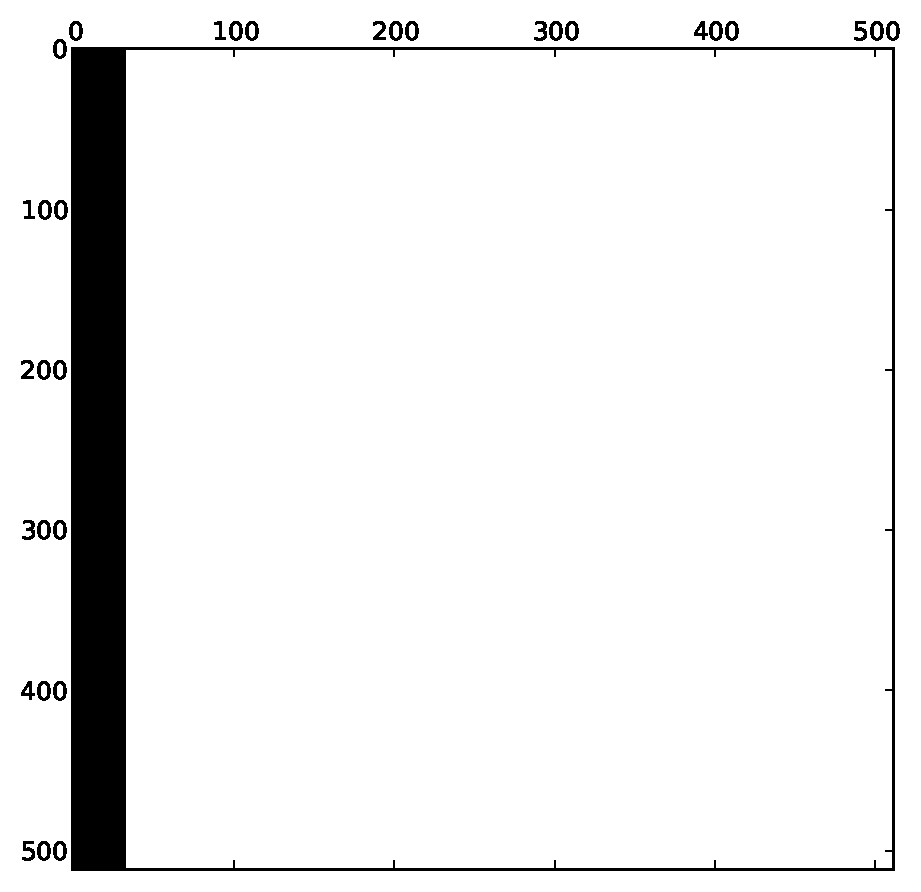
\includegraphics[width=\ww]{figures/supercompact_matrix-crop.pdf}}%
    \subfigure[Compact.]{%
    \label{fig:compact}
	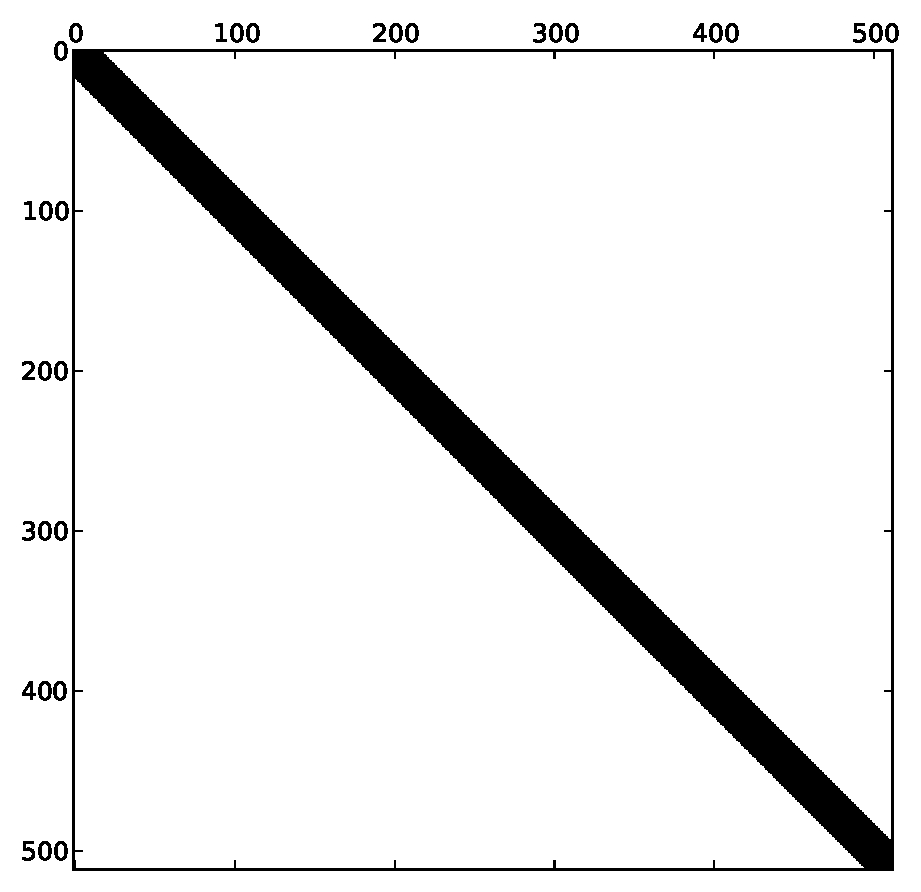
\includegraphics[width=\ww]{figures/compact_matrix-crop.pdf}}%
    \subfigure[Random.]{%
    \label{fig:random}
	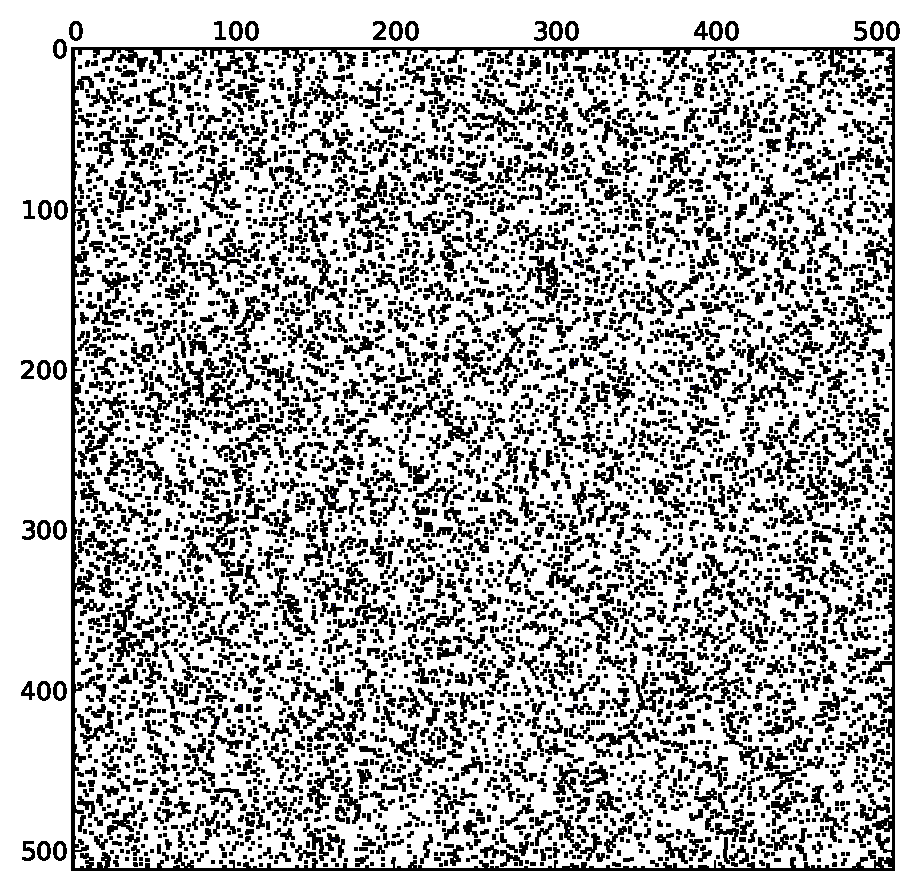
\includegraphics[width=\ww]{figures/random_matrix-crop.pdf}}%
    \end{center}
	\caption{Different sparsity distributions. In all cases, there are 32 nonzeros per line and 300 rows.}
\end{figure}

\def\ww{.20\textwidth}
\begin{figure}
\begin{center}
    \subfigure[2D, no RCM.]{%
    \label{fig:supercompact}
	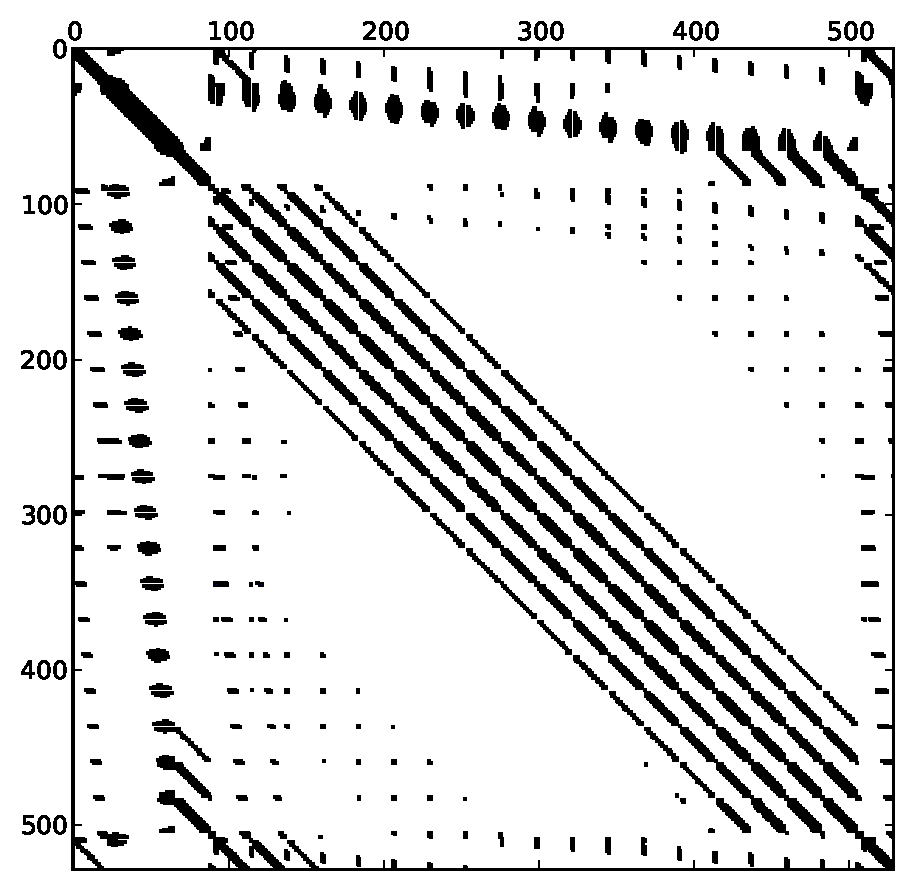
\includegraphics[width=\ww]{figures/kd-tree-2d-norcm-crop.pdf}}%
    \subfigure[2D, RCM.]{%
    \label{fig:compact}
	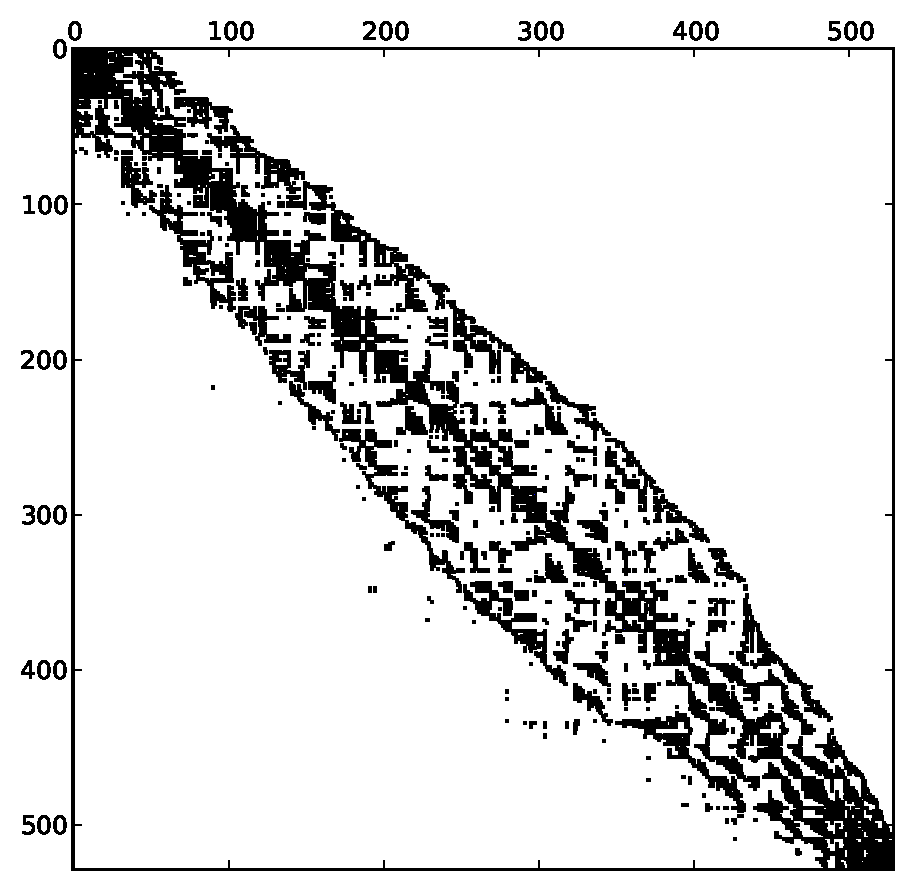
\includegraphics[width=\ww]{figures/kd-tree-2d-rcm-crop.pdf}} \linebreak
    \subfigure[3D, RCM.]{%
    \label{fig:random} 
	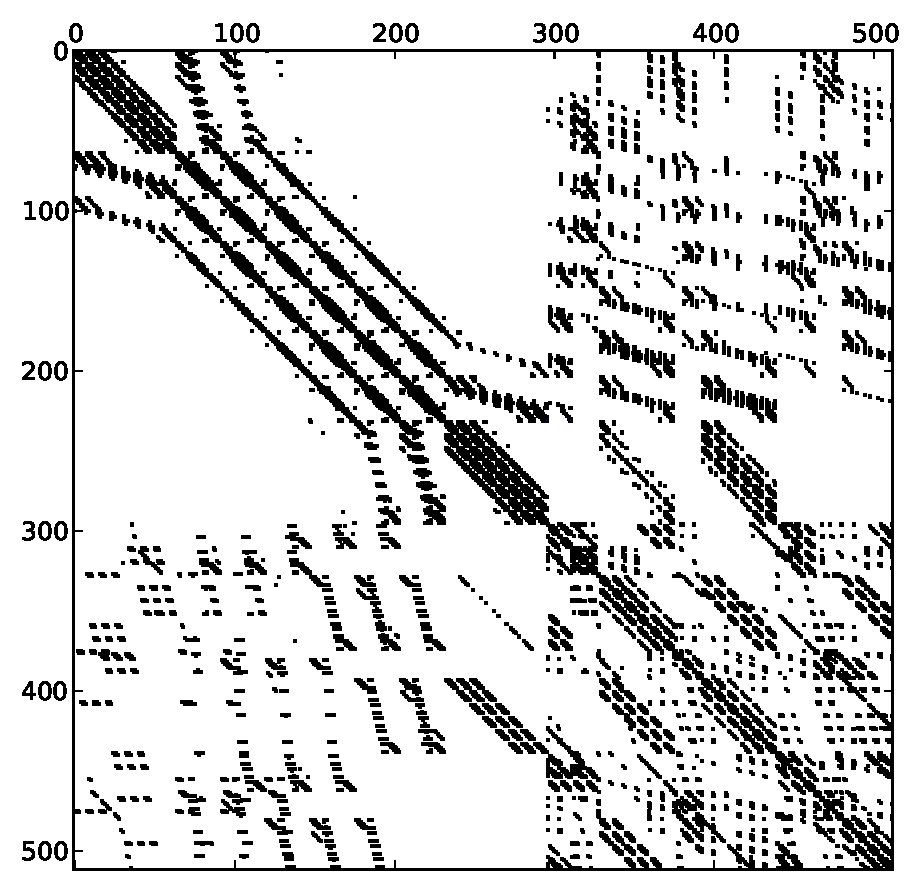
\includegraphics[width=\ww]{figures/kd-tree-3d-norcm-crop.pdf}}%
    \subfigure[3D, RCM.]{%
    \label{fig:random}
	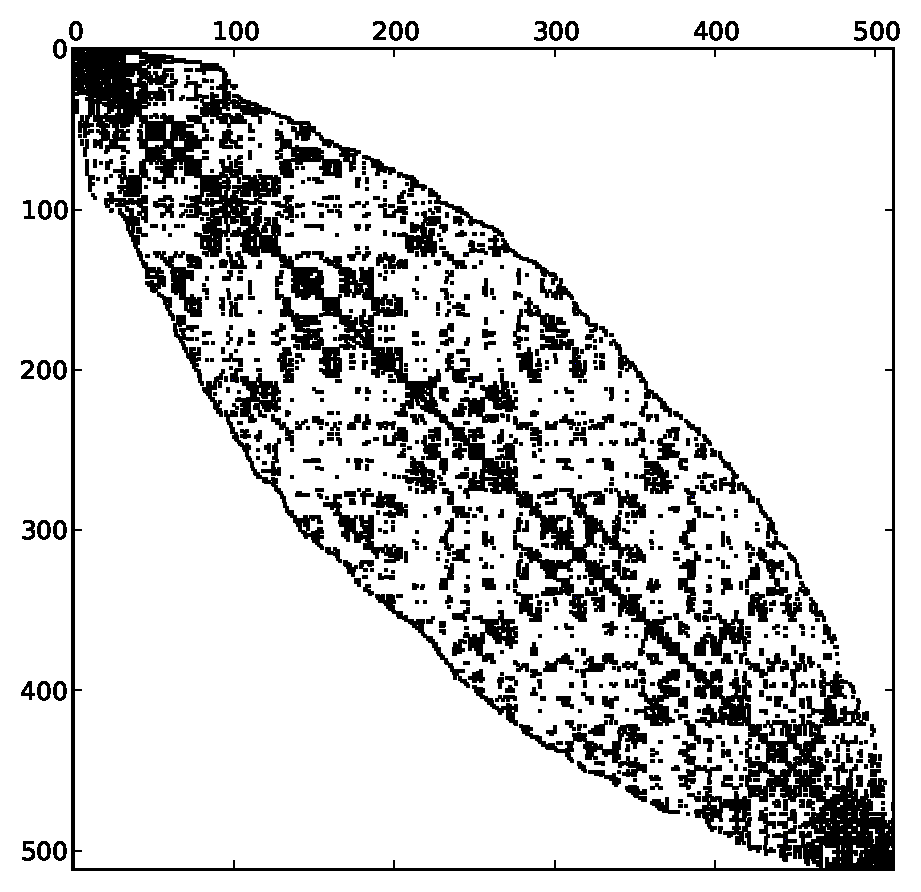
\includegraphics[width=\ww]{figures/kd-tree-3d-rcm-crop.pdf}}%
    \end{center}
	\caption{Matrix A that corresponds to derivative stencils in 2D (a-b) and 3D (c-d) 
      RBF-FD calculations.}
\end{figure}

